%!TEX root = ../main.tex



\section{Αρχιτεκτονική}

Το Visfx είναι μία επεκτάσιμη και κατανεμημένη πλατφόρμα δημιουργίας αναλυτικών και απεικόνισης δεδομένων. Στην παρούσα υλοποίηση χρησιμοποιείται για να βοηθήσει έναν μηχανικό ο οποίος μπορεί να δουλεύει σε μία εταιρεία συναλλάγματος στη δημιουργία ενός συστήματος συστάσεων νομισματικών ζευγών· θα μπορούσε όμως να χρησιμοποιηθεί και για αρκετά διαφορετικά σενάρια. Χρησιμοποιώντας το Visfx μπορεί κανείς να αποθηκεύσει σετ δεδομένων, να κάνει αναζητήσεις και υπολογισμούς πάνω σ' αυτό, καθώς και να απεικονίσει τα αποτελέσματα του με τη μορφή μίας ιστοσελίδας. 

Η πλατφόρμα τρέχει σε κάποιον απομακρισμένο σέρβερ—ή σέρβερς—και αποτελείται από τρεις βασικές μονάδες, οι οποίες υλοποιούν και ένα διαφορετικό κομμάτι του Visfx. Κάθε μονάδα αποτελείται από ανεξάρτητους (υπό-)σέρβερ που υλοποιούν μία συγκεκριμένη λειτουργεία οι οποίοι επικοινωνούν μεταξύ τους. Το Visfx είναι φτιαγμένο με τέτοιο τρόπο ώστε να περιέχει όλες τις εξαρτήσεις του κάνοντάς την εγκατάστασή του μία πολύ απλή υπόθεση. Οι μονάδες από τις οποίες αποτελείται το Visfx είναι:
\begin{itemize}
	\item τη μονάδα Αποθήκευσης και Ανάκτησης Δεδομένων
	\item τη μονάδα Επεξεργασίας και Δημιουργίας Αναλυτικών
	\item και τη μονάδα Παρουσίασης και Απεικόνισης των Δεδομένων.
\end{itemize}

\begin{figure}[H]
  \centering
  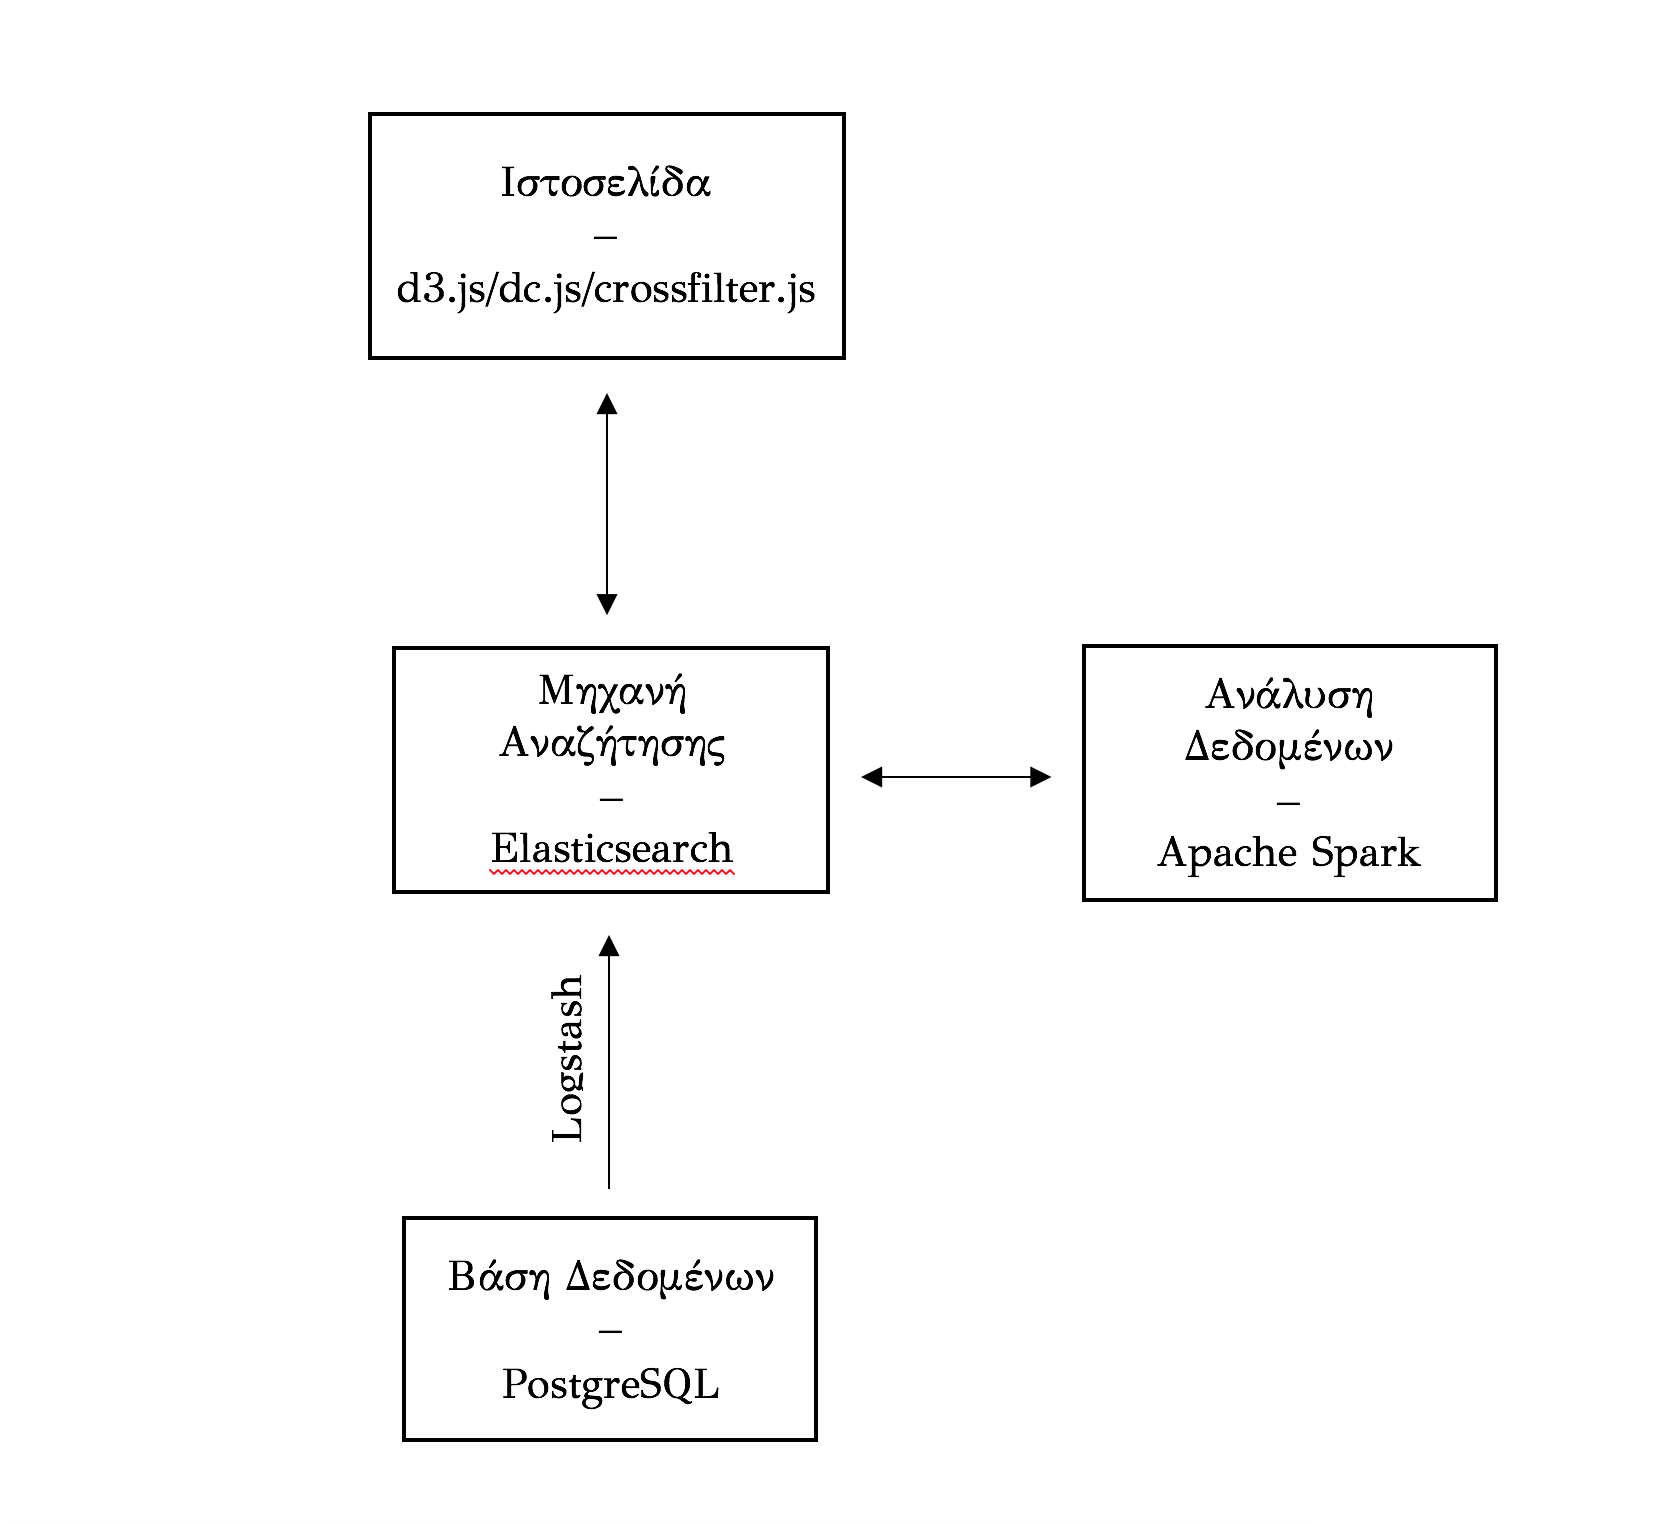
\includegraphics[width=\textwidth]{architecture}
  \label{fig:architecture}
\end{figure}

Τα δεδομένα 

\section{Docker}

Το Visfx είναι φτιαγμένο χρησιμοποιώντας το Docker. Το Docker είναι 

\section{Αποθήκευση και ανάκτηση Δεδομένων}
\subsection{PostgreSQL}
\subsection{Elasticsearch \& Logstash}

\section{Ανάλυση Δεδομέων}

\section{Παρουσίαση \& Απεικόνιση δεδομένων}
\subsection{d3.js, dc.js, crossfilter.js}